\section{Visión Artificial} \label{sect:Vision_Artificial}

Una manera de obtener información del ambiente es con la visión artificial. Esta consiste en usar un dispositivo (cámara) que capta un rango de espectro electromagnético y produce una imagen. La representación de la imagen se almacena como una matriz de píxeles, cada píxel es un elemento que guarda información de una región en el espacio captado. Si se usa una cámara de luz, la información de cada píxel será el color. \cite{AiRobotics}  

Por lo general luego de obtener una imagen se requiere extraer información de ella, por lo cual se han desarrollado diferentes algoritmos y t\'ecnicas que ayudan en esta tarea. En la sección \ref{sec:Segmentacion} se describe la t\'ecnica de segmentaci\'on por regiones, que es la utilizada en el proyecto. 

Por otro lado, existen varios algoritmos que se dedican a la transformación de las imágenes para reducir
ruidos, compensar problemas de iluminación, extraer formas, identificar objetos, entre otros. En esta sección se describen dos de las técnicas de transformación para reducir el ruido basadas en la dilatación y erosión de la imagen (secci\'on \ref{sec:Transfor}). 
 
\subsection{Segmentaci\'on por regiones}\label{sec:Segmentacion}

La técnica de segmentación por regiones consiste en identificar un conjunto de píxeles adyacentes entre sí que compartan un rango de colores establecidos. Generalmente, en robótica luego de identificar esa zona se ubica el centro y se navega hasta él \cite{BookOpenCv}. 

\subsection{Filtros}
El filtrado de imágenes es una técnica para la transformación de imágenes, que consiste en destacar  sus características más relevantes en base a un propósito en particular. 

Generalmente en la tarea de extracción de información de una imagen se utilizan filtros para descartar zonas o características que no son importantes para el patrón deseado y para determinar el área deseada ya sea por patrones de forma o color.

Por otro lado, existen transformaciones morfológicas que se utilizan en una amplia variedad de contextos como la eliminación del ruido, aislamiento de elementos individuales y elementos de unión dispares en una imagen. Algunas de las transformaciones básicas son: dilatación, erosión, uni\'on e intersecci\'on \cite{BookOpenCv}.

En esta investigación, los algoritmos de filtrado aplicados a las imágenes fueron: Clausura Morfológica y Apertura Morfológica, filtros que aplican las transformaciones morfológicas de erosión y dilatación a las imágenes.

%\subsection*{Transformaciones Morfológicas}\label{sec:Transfor}
 

\subsubsection{Dilatación}
La dilatación es una convulsión (patr\'on que se le aplica a toda la imagen) entre una imagen (o región de una imagen), que llamaremos $A$ y un núcleo que llamaremos $B$. El n\'ucleo es una plantilla o m\'ascara de cualquier forma o tamaño, implementado como una matriz, de tamaño fijo, de coeficientes numéricos. De los elementos de la matriz se define uno como punto de anclaje, que normalmente se encuentra en el centro. La convulción se aplica calculando el m\'aximo valor de los píxeles de la imagen común a $B$ y se reemplaza el píxel de la imagen en el punto de anclaje con ese valor máximo. Esto causa regiones brillantes dentro de una imagen y la hace crecer. Este crecimiento es el origen del término `` operador de dilatación" \cite{BookOpenCv}. 

\begin{figure}[hbtp]

\centering
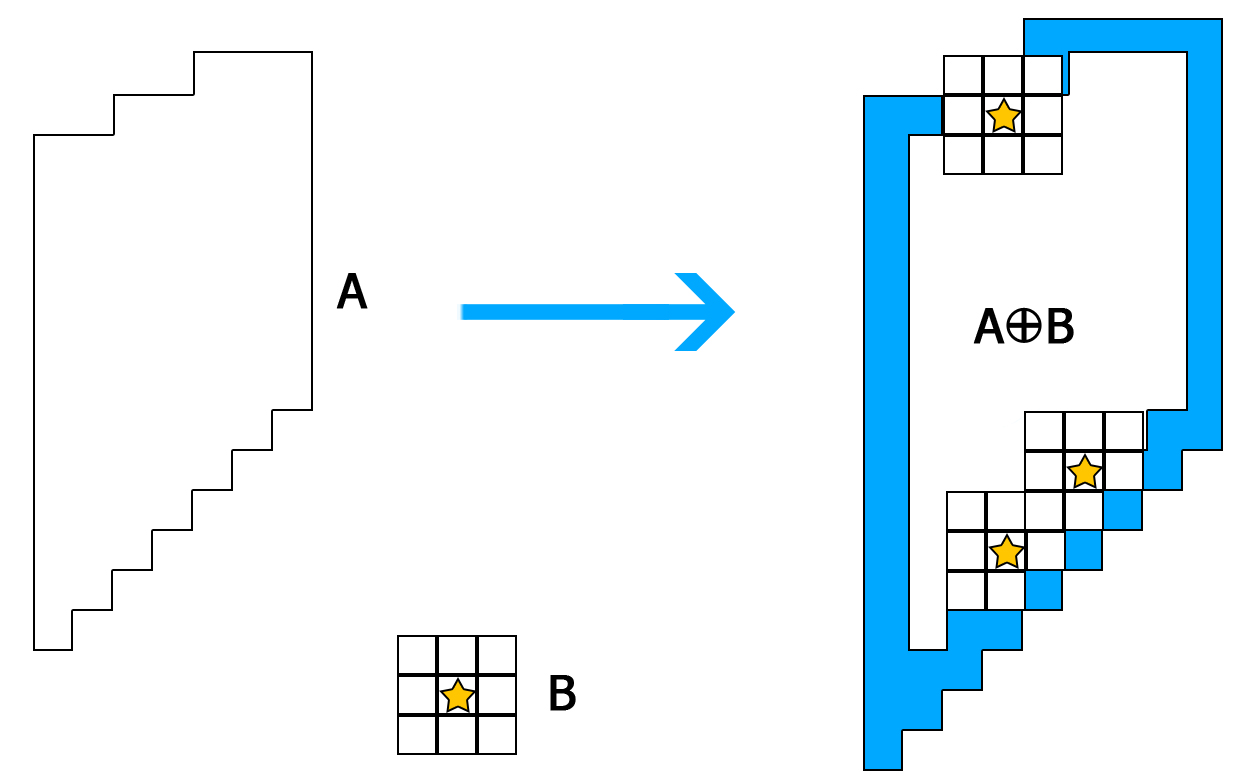
\includegraphics[scale=0.2]{imagenes/erosion-model.jpg}
\caption{Dilatación A: es la imagen original, B: es el n\'ucleo, La estrella es el punto de referencia. Se ve como aumenta la imagen en proporci\'on al patr\'on aplicado }
\end{figure}

\subsubsection{Erosión}
La erosión es la operación inversa a la dilatación. Esta acción del operador es equivalente a el cálculo de un mínimo local sobre el área del núcleo. La erosión genera una nueva imagen a partir de la original, utilizando el siguiente algoritmo: como el núcleo $B$ es analizado sobre la imagen, se calcula el mínimo valor del píxel superpuesto por $B$ y se reemplaza el píxel de la imagen con un punto de referencia de valor mínimo \cite{BookOpenCv}. 
V\'ease en la figura \ref{fig:erosion}

\begin{figure}[hbtp]
\centering
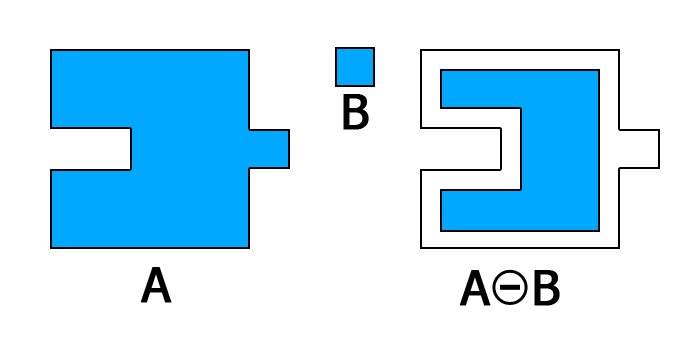
\includegraphics[scale=0.3]{imagenes/erosion.jpg}
\caption{Erosión,  A: es la imagen original, B: es el n\'ucleo, La estrella es el punto de referencia. Se ve como disminuye la imagen en proporci\'on al patr\'on aplicado}
\label{fig:erosion}
\end{figure}

Este cap\'itulo constituyo la base te\'orica que sustenta el proyecto, en el siguiente cap\'itulo se presenta el proceso de desarrollo que se sigui\'o para su culminaci\'on. 
